\documentclass[a4paper, 11pt, titlepage]{jsarticle}
\usepackage[dvipdfmx]{graphicx}

\title{メモリ消費による実行速度の影響}

\author{235718G 新里 伊武輝 }
\date{\today}

\begin{document}
\maketitle

\clearpage

\section{実行結果}
メモリを大量に消費した際の実行結果は図\ref{fig:1}と図\ref{fig:2}に示す。

\begin{figure}[htbp]
    \centering
    \begin{minipage}{0.45\textwidth}
        \centering
        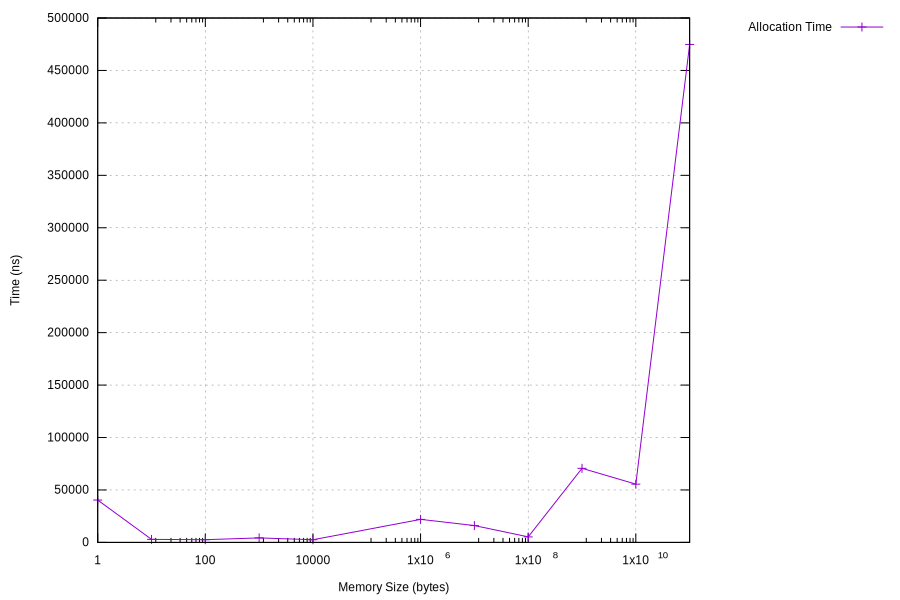
\includegraphics[width=\linewidth]{../img/malloc_plot_macos.pdf}
        \caption{localでの実行結果}
        \label{fig:1}
    \end{minipage}
    \hfill
    \begin{minipage}{0.45\textwidth}
        \centering
        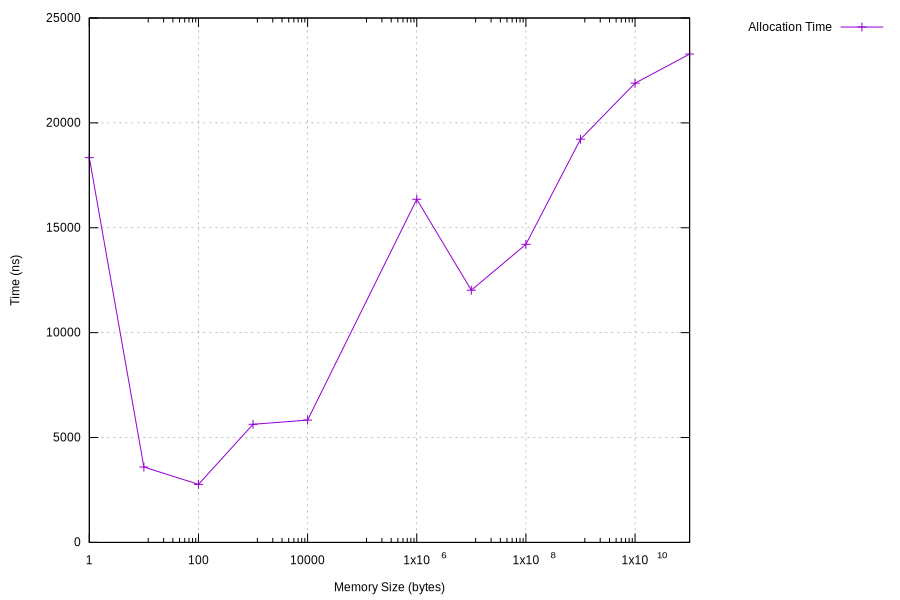
\includegraphics[width=\linewidth]{../img/malloc_plot_linux.pdf}
        \caption{amaneでの実行結果}
        \label{fig:2}
    \end{minipage}
\end{figure}


\section{考察}
図\ref{fig:1}と図\ref{fig:2}の共通部分として、消費するメモリの量が多ければ多いほど実行時間が長くなることがわかる。特に、メモリ量が少なすぎるとシステムのオーバーヘッドが増大し、割り当てやキャッシュミスが発生するため、逆に処理が遅くなる可能性がある。さらに、localとamaneでは、amaneの方が使用可能なメモリ量が多く、システム自体のメモリ速度やプロセッサの性能により、同じメモリ量の消費でも処理速度がかなり速いことが確認できる。


\end{document}
